This section section describes the results of different measurements, calculations and tests that were run on the Barricelli computer.
It also documents the different demonstration programs that showcase and illustrate Barricelli's purpose through practical use.

\section{Measurements}

\subsection{Performance}

\todo{measure performance with different core amounts}

\todo{measure performance with and without genetics pipeline}

\todo{measure performance of same problems on consumer grade laptop}

\todo{measure performance of general program}

\subsection{Energy Efficiency}

\todo{measure power usage (idle, working, etc)}

\section{Demonstration Programs}

This section documents the demonstration programs written for the Barricelli computer to demonstrate its functionality.
The programs are typically written in \gls{galapagos} assembly for programs running on the custom processor, and C for programs running on the \Gls{SCU}.
The source code for these demonstration programs can be found in appendix \vref{appendix:demonstration-programs-source-code}.

\subsection{Genetic Algorithm: Color Search}

The color search program is a very simple program demonstrating a basic usage of the genetics accelerator.
The program tries to find a specific color in the search-space of all 24-bit colors.

\subsubsection{Individual representation}

An individual represents a specific 24-bit color in RGB format.
The individual is coded to a 64-bit data word like in figure \vref{figure:color-search-bytefield}.

\begin{figure}[H]
    \begin{center}
        \begin{bytefield}[bitwidth=0.5em,endianness=big]{64}
            \bitheader[bitformatting={\tiny\rotatebox[origin=B]{90}}]{0, 7, 8, 15, 16, 23, 24, 63} \\
        \bitbox{40}{\color{lightgray}\rule{\width}{\height}}
            \bitbox{8}{blue}
            \bitbox{8}{green}
            \bitbox{8}{red}
        \end{bytefield}
        \caption{The binary coding of an individual for the color search problem}
        \label{figure:color-search-bytefield}
    \end{center}
\end{figure}

\subsubsection{Fitness Function}

The fitness for an individual is calculated using equation \vref{equation:color-search-fitness-function}.
The fitness a any given individual falls in the range $ [0, 768] $.

\begin{eqnarray}
\nonumber
fitness & = & 768 \\
\nonumber
        & - & |red_{individual} - red_{target}| \\
\nonumber
        & - & |green_{individual} - green_{target}| \\
        & - & |blue_{individual} - blue_{target}|
\label{equation:color-search-fitness-function}
\end{eqnarray}

\subsubsection{Results}

Figure \vref{figure:color-search} shows the evolution of the approximation suggested as an answer by the genetic algorithm.
In this problem instance the target color was magic pink, i.e. the color with color code $ rgb(255, 0, 255) $.
The program run illustrated in figure \vref{figure:color-search} ran on 7 seven cores, and the measurements are from regularly polling a single core for its current best solution.
Figure \vref{figure:color-search} clearly illustrates a typical trait of genetic algorithm approximations: they are quite good at finding decent approximations, but iterating to improve accuracy of the result is a game of diminishing returns.
The algorithm quickly finds a decent approximation of the target color, but finding the exact value down to the last bit still takes time.

\begin{figure}[H]
    \begin{center}
        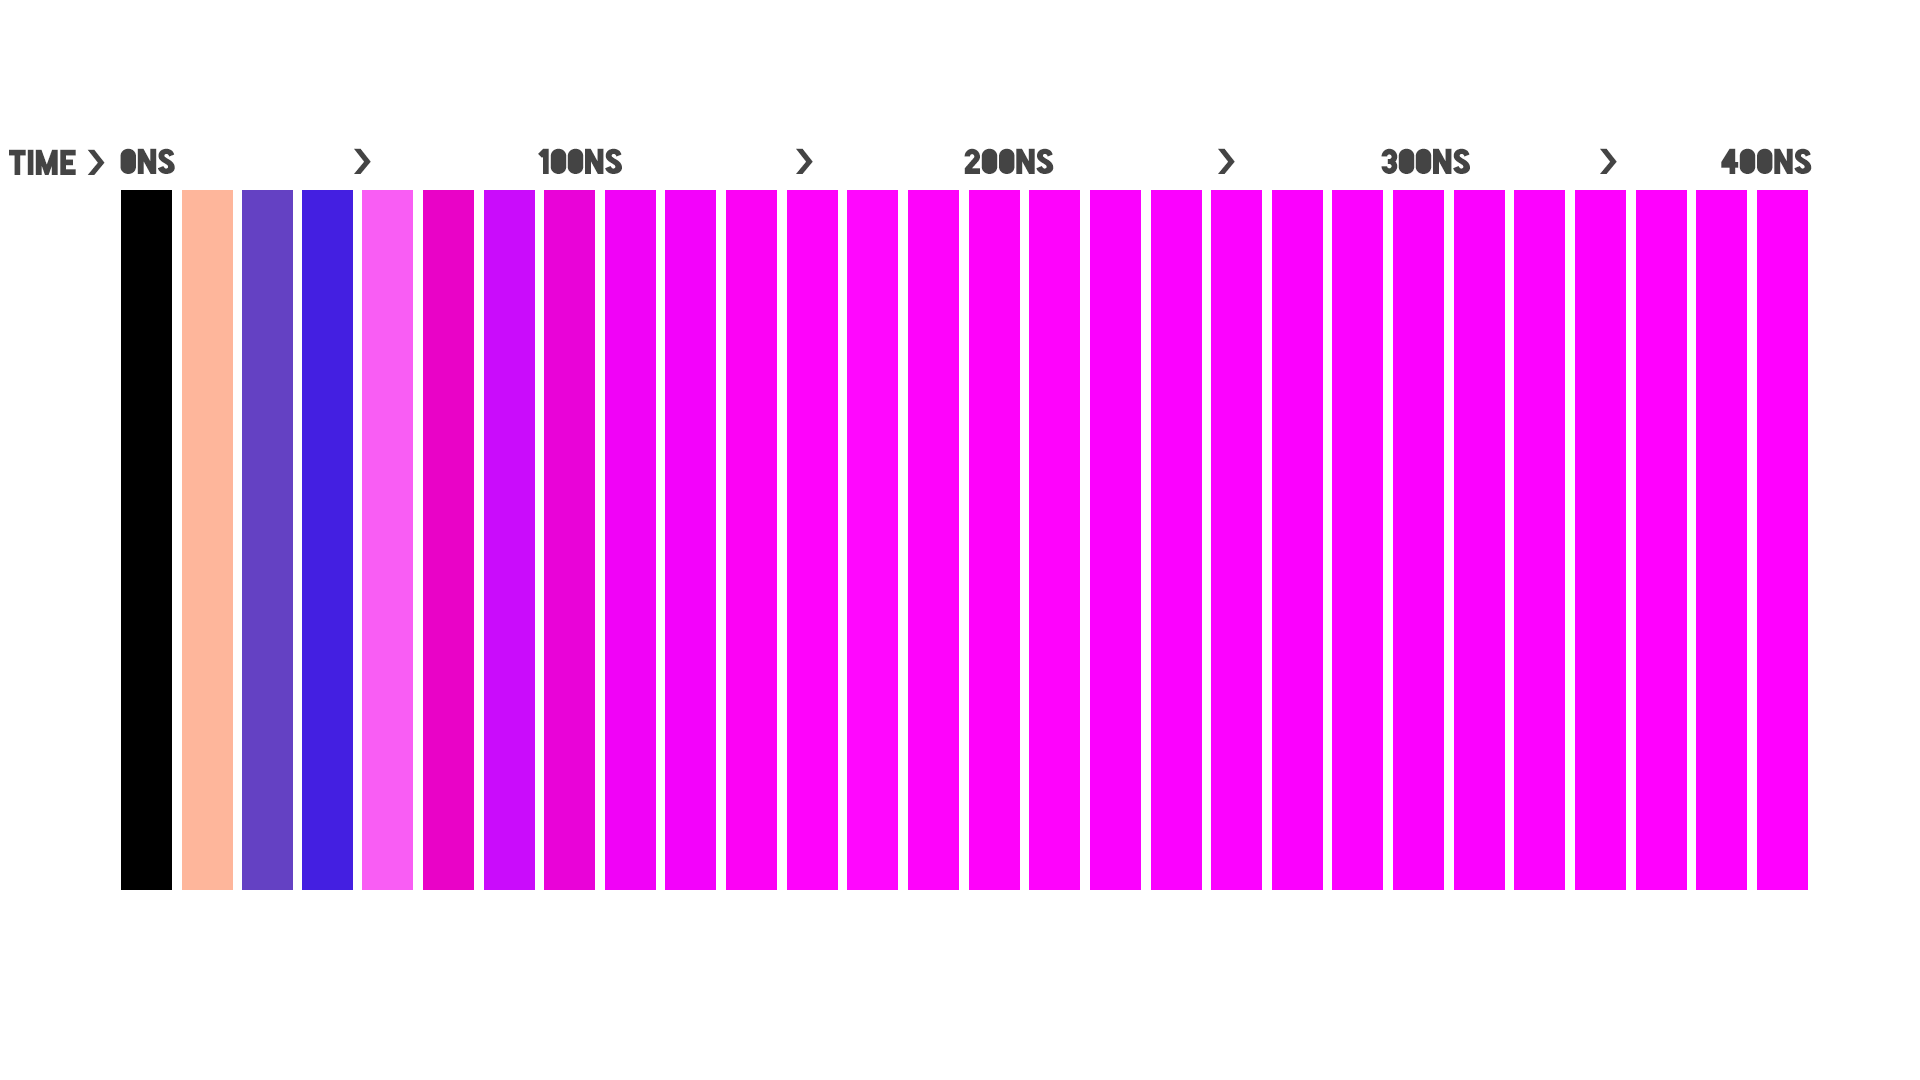
\includegraphics[width=\textwidth]{fig/color-search}
    \caption{Color search progression (7 cores, 1 core sampled)}
    \label{figure:color-search}
    \end{center}
\end{figure}

\subsection{Genetic Algorithm: Binary Knapsack Problem}

\todo{Explain the binary knapsack program}
The binary knapsack problem is an optimization problem that is considered NP-hard. The algorithm aims to find the best resource allocation given a set of items and their weight. The solution of the problem can be seen as putting a set of elements in an knapsack. The goal is to find the best possible combinations of elements to put in the knapsack. E.g  a set of elements that yield the best resource allocation. This is achieved by putting the different combination through an evolutionary process. For each possible solution is considered by calculating the fitness value. 

\todo{Someone finish this please}  






\subsubsection{Individual representation}

An individual represents a \todo{...}.
The individual is coded to a 64-bit data word like in figure \vref{figure:binary-knapsack-bytefield}.

\begin{figure}[H]
    \begin{center}
        \begin{bytefield}[bitwidth=0.5em,endianness=big]{64}
            \bitheader{0, 63} \\
            \bitbox{63}{bit $ i $ set if item $ i $ is in the include set, else unset}
        \end{bytefield}
        \caption{The binary coding of an individual for the binary knapsack problem}
        \label{figure:binary-knapsack-bytefield}
    \end{center}
\end{figure}

\subsubsection{Fitness Function}

The fitness for an individual is calculated using equation \vref{equation:binary-knapsack-fitness-function}.
The fitness a any given individual falls in the range \todo{a range}.

\begin{eqnarray}
\nonumber 
fitness & = & \\
        &   & \todo{a fitness function}
\label{equation:color-search-fitness-function}
\end{eqnarray}

\subsubsection{Results}

\todo{results}

\subsection{Blinkenlights}

Blinkenlights is a program that demonstrates the use of the input and output of the \Gls{barricelli} driven by the \Gls{SCU}.
Blinkenlights blinks the 16 output LEDs of the computer and can react to button presses.

\todo{somebody needs to write this program.}
